Neural networks are a method for statistical machine learning. The network takes as input n-dimensional vector $\vec{i} = (i_1, i_2, ..., i_n)$ and produces an m-dimensional output $\vec{o} = (o_1, o_2, ...o_m)$. A neural network is defined by several layers of neurons, where each neuron is connected to every neuron in the layer before and after it (see figure \ref{fig:ANN}). Each of these connections has an associated weight, and each neuron holds a value. Let us denote the value of a neuron $i$ in layer $j$ as $x_{i,j}$ and the weight for the connection between layer $x_{i,j}$ and $x_{k, j+1}$ as $w_{i,k,j}$. Each layer also has an activation function $\sigma$, such that 

\begin{equation}
x_{k,j+1} = \sigma (b_{k,j+1} + \sum_{i} w_{i,j,k} \cdot x_{i, j}) 
\end{equation}

where $b_{i,j}$ is the bias term for neuron $x_{i,j}$ \cite{feedForwardApprox}. 
The value of the neuron $x_{k,j+1}$ is then the activation function applied to the sum of all the values in the layer before multiplied by their respective weights. Then network is said to "feed-forward", since the next layer is inferred from the previous layer. The first layer of neurons will contain $n$ neurons, representing the input $\vec{i}$, which will feed-forward until they reach the $m$ neurons in the final layer, the output $\vec{o}$. Hornik showed that a neural network with 3 layers (input, output and one more "hidden" layer in between) and enough neurons in each layer can approximate any continuous function over some bounds within some error margin, regardless of the choice of activation function \cite{feedForwardApprox}. Adding more neurons or more layers will (on average) improve accuracy, but it does this at the cost of computational performance. The number of layers and the number of neurons in each layer are then hyperparameters, which themselves need to be optimized by the designer of the network in order to find a suitable architecture for the problem at hand. This is often done via a grid-search approach. The rectified linear or relu activation function is often used in practice as it is computationally cheap, 

\begin{equation} \sigma(x) = \begin{cases} 
      0 & x \leq 0 \\
      x &  x > 0 \\
   \end{cases}
\end{equation}


\begin{figure}
\centering
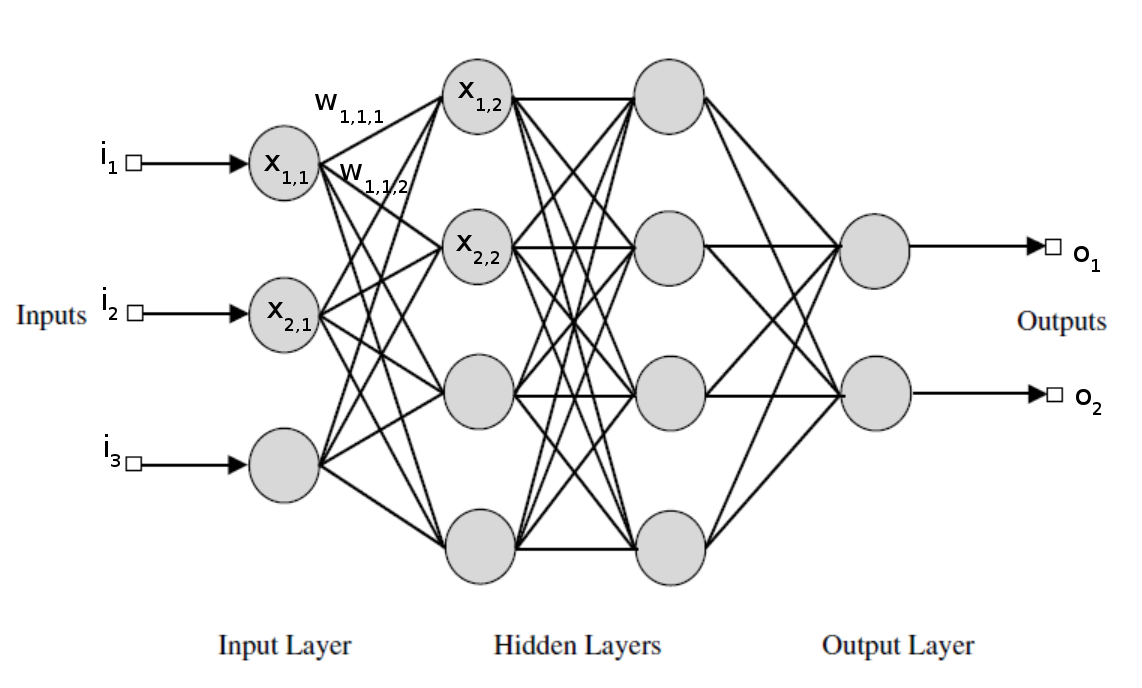
\includegraphics[scale=0.32]{pictures/ANN}
\caption{The architecture of a feed-forward neural network with 4 layers \cite{natureOfCode}}
\label{fig:ANN}
\end{figure}

